\chapter{Introducción Específica}\label{Chapter2}

\section{Requerimientos}

\begin{enumerate}
    \item Verificación
    \begin{enumerate}
        \item \textit{Tests} unitarios de cada módulo funcional.
        \item Simulación de bloques de protocolo completos.
        \item Simulación del sistema completo haciendo \textit{loopback} entre el trasmisor y el receptor.
    \end{enumerate}
    % \item Validación
    % \begin{enumerate}
    %     \item Medición y observación de audio y video luego de pasar por el sistema completo.
    %     \item Medición de los los paquetes con un analizador según la norma.
    %     \item Cumplir con el bitrate de los estándares dentro del rango de SD-SDI y 3G-SDI.
    % \end{enumerate}
    \item Funcionalidad
    \begin{enumerate}
        \item Obtener las tasas de datos contempladas dentro del rango de los normas SD-SDI y 3G-SDI\@.
        \item Obtener un diseño sin problemas de \textit{timing} en las señales entre dominios de reloj
        dentro del módulo.
        \item Obtener un módulo sin problemas de \textit{timing} por \textit{setup} o \textit{hold} en las señales de entrada y salida.
        \item La implementación del sistema no debe ocupar más del 3000 \textit{Logic Array Blocks} en la FPGA\@.
    \end{enumerate}
    \item Metodologı́a de trabajo
    \begin{enumerate}
        \item Control de versiones mediante SVN o Git.
        \item Desarrollo en Quartus con licencias para análisis de \textit{timing} y simulaciones o herramientas \textit{open source}.
        \item Planificación y documentación mediante Redmine o Gitlab.
        \item Diseño modular.
    \end{enumerate}
    \item Documentación
    \begin{enumerate}
        \item Confección de la memoria técnica.
        \item Confección de documentación del diseño del módulo.
        \item Confección de documentación de uso del módulo.
    \end{enumerate}
\end{enumerate}

\section{Estructura general del sistema y diagrama en bloques}

En cuanto a la implementación en FPGA, la interfaz SDI consta de dos capas
independientes, que se pueden visualizar en la figura~\ref{fig:sdi}, la de
recepción/transmisión y la de protocolo, por tal motivo el módulo deberá
implementar ambas instancias de manera separada. Para la primera, se suelen
usar \textit{hard-transceivers}, contenidos en la FPGA o \textit{soft-transceivers}
instanciados en la lógica programable, para las aplicaciones con menor demanda
de tasa de datos. Este módulo se puede encargar de muestrear la entrada
asincrónica, sincronizarse a la misma y deserializar los datos, para casos más
exigentes es necesario usar un \textit{hard-transceivers}. En este diseño no se
pretende resolver esta parte del desarrollo, sino usar las soluciones que
proporcionan los fabricantes de los dispositivos, que por lo general son de uso
libre, aunque propietarias. El desarrollo que puede ser necesario dependiendo
el fabricante que se elija es el controlador de dicho módulo.

Para la segunda etapa, se debe implementar un submódulo que trabaje en el dominio
de los datos paralelizados y tenga la información propia del protocolo para
interpretar, acondicionar y validar la señal. Esta parte del desarrollo se
encarga principalmente de la sincronización de paquetes y de la detección de
errores. Aunque la interfaz funciona en un solo sentido a la vez, debe ser
configurable para funcionar como transmisor y receptor de manera separada, como
se ilustra en la figura~\ref{fig:sdi}. Por lo tanto, el módulo debe ser capaz
de tomar la señal serie que llega a la FPGA desde el \textit{driver} del cable,
deserializarla y procesarla en un sentido y empaquetarla la señal acorde al
protocolo y serializarla en el otro sentido.

\vspace{1cm}
\begin{figure}[htbp]
    \centering
    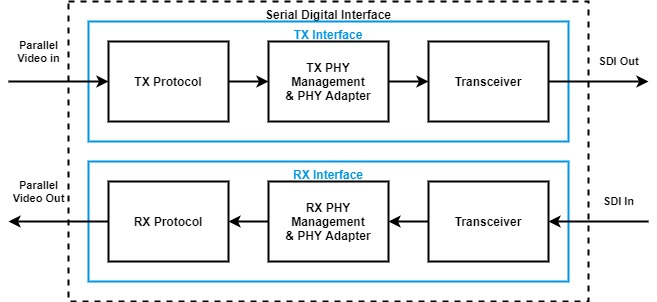
\includegraphics[width=\linewidth]{./Figures/sdi.jpg}
    \caption{Diagrama en bloques general de interfaz digital serie}\label{fig:sdi}
\end{figure}
\vspace{1cm}

\documentclass{article}
\usepackage[utf8]{inputenc}
\usepackage{enumitem}

\section{Estándares soportados por la interfaz}

El módulo soporta SMPTE SD/HD/3G-SDI implementa tres estándares de la interfaz:

\begin{itemize}[label=--]
    \item SD-SDI (SMPTE ST 259): Señal digital de televisión estándar.
    \item HD-SDI (SMPTE ST 292\-1): Interfaz serie de señal de 1.5 Gb/s.
    \item 3G-SDI (SMPTE ST 424): Interfaz serie de señal de 3 Gb/s.
\end{itemize}

\subsection{Definición estándar}

El módulo está diseñado para soportar la tasa de bits de 270 Mb/s y es compatible
con el estándar de detección y manejo de errores o EDH (del inglés, Error
Detection and Handling) SMPTE RP 165 para las secciones de recepción y transmisión.

\subsection{Alta definición}

Aunque el estándar se llama interfaz de 1.5 Gb/s, las tasas de bits admitidas
por HD-SDI es en realidad de 1.485 Gb/s y 1.485/1.001 Gb/s. El módulo es
compatible con ambas tasas de bits y con la generación (transmisor) y
verificación (receptor) de valores CRC (del inglés, Cyclic Redundancy Check)
para cada línea de video, así como la inserción (transmisor) y captura (receptor)
de valores de número de línea para cada línea.

\subsection{Ultra alta definición}

Como con el estándar anterior, llama interfaz de 3 Gb/s, pero las tasas de bits
real es de 2.97 Gb/s y 2.97/1.001 Gb/s. El módulo es compatible con ambas tasas
de bits. 3G-SDI admite varios niveles de mapeo diferentes, descritos en el
estándar SMPTE ST 425\-1. El núcleo es compatible con todos estos niveles. Al
igual que con el estándar HD-SDI, el núcleo también es compatible con la
generación y verificación de CRC, así como la inserción y captura de números de
línea para 3G-SDI\@.

\subsection{Identificación de carga útil y soporte de datos auxiliares}

El módulo implementa una capacidad de inserción de paquetes de datos auxiliares
de identificación de carga útil SMPTE ST 352 para el transmisor que funciona en
todos los 3 modos SDI ya mencionados. El lado receptor también detecta y captura
los cuatro bytes de datos de los paquetes de identificación de carga útil ST 352.

Además, implementa la inserción de paquetes de datos auxiliares antes de la
transmisión. Aunque módulo no proporciona una capacidad de inserción de paquetes
de datos auxiliares, excepto para los paquetes de identificación de carga útil
ST 352, tiene puertos de datos necesarios para permitir que la inserción de
paquetes de datos auxiliares sea implementada por el usuario. En el lado del
receptor, todos los datos auxiliares insertados son preservados por el receptor.
El módulo pueden procesar el flujo de datos SDI recibidos y/o modificar los datos
auxiliares según sea necesario.

\section{Submódulos del sistema}

